\documentclass[10pt]{article}
\usepackage[top=2cm,bottom=2cm,left=2cm,right=2cm]{geometry}
\usepackage[dvipsnames,svgnames,x11names]{xcolor}
\usepackage{multicol}
\usepackage{graphicx}
\usepackage{amsmath,amssymb,amsfonts}
\usepackage{booktabs}
\usepackage{colortbl}
\usepackage{multirow}
\usepackage{tcolorbox}
\usepackage{enumitem}
\usepackage{titlesec}
\usepackage{float}
\usepackage{hyperref}
\usepackage{tabularx}
\usepackage{subcaption}
\setlength{\parindent}{0pt}
\setlength{\parskip}{6pt}

\graphicspath{{architecture/}}

\begin{document}

%% ============================================================
%% TITLE
%% ============================================================
\begin{center}
{\LARGE\bfseries Structured Knowledge-Enhanced Retrieval for Financial Documents}\\[4pt]
{\large\bfseries Truy xuất tài liệu tài chính tăng cường cấu trúc tri thức}\\[8pt]
{\large Đề xuất nghiên cứu}\\[6pt]
\textit{Benchmark:} $\mathrm{T}^{2}$-RAGBench (EACL 2026) --- FinQA $\cdot$ ConvFinQA $\cdot$ TAT-DQA
\end{center}

\vspace{4pt}
\hrule
\vspace{8pt}

%% ============================================================
%% TÓM TẮT
%% ============================================================
\section*{Tóm tắt}

Truy xuất ngữ cảnh chính xác từ các báo cáo tài chính hỗn hợp văn bản và bảng biểu là một bước then chốt trong các hệ thống RAG cho lĩnh vực tài chính. Các phương pháp truy xuất hiện tại gặp khó khăn do bỏ qua các đặc trưng ngôn ngữ và ràng buộc toán học vốn có của tài liệu tài chính. Bài báo này phân tích bốn hiện tượng nền tảng gây ra thất bại của các retriever thông thường: tính thể loại đặc thù, ảo tưởng trùng lặp từ vựng, mất nhất quán toán học và bất ngờ ngữ nghĩa. Từ đó, chúng tôi đề xuất GSR (Graph-Structured Retrieval) -- một phương pháp biểu diễn bảng tài chính dưới dạng đồ thị tri thức với các cạnh ràng buộc kế toán, kết hợp với cơ chế chấm điểm nhận biết ràng buộc. Để huấn luyện, chúng tôi phát triển CACL (Constraint-Aware Contrastive Learning) và kỹ thuật sinh mẫu âm CHAP dựa trên phá vỡ có chủ đích các đẳng thức kế toán. Nghiên cứu này thực nghiệm trên bộ benchmark cho miền dữ liệu tài chính tiêu chuẩn $\mathrm{T}^{2}$-RAGBench.

%% ============================================================
%% 1. GIỚI THIỆU
%% ============================================================
\section{Giới thiệu}

Truy xuất ngữ cảnh phù hợp từ kho tài liệu tài chính (báo cáo thường niên, báo cáo quý) là bài toán nền tảng cho các hệ thống sinh tăng cường truy xuất (RAG) trong lĩnh vực này. Đầu vào là một câu hỏi tài chính $Q$ và một kho gồm $N$ tài liệu $\{D_1, \ldots, D_N\}$, mỗi tài liệu chứa văn bản tự sự, bảng dạng markdown và siêu dữ liệu (tên công ty, năm báo cáo, ngành). Đầu ra là danh sách top-$K$ tài liệu liên quan nhất, đánh giá qua các chỉ số MRR@3, Recall@1/3/5, NDCG@3 theo chuẩn của $\mathrm{T}^{2}$-RAGBench~\cite{strich2026t2ragbench}.

Thách thức chính nằm ở tính chất hỗn hợp của thông tin tài chính: câu trả lời thường đòi hỏi kết hợp cả văn bản lẫn bảng số liệu. Các hệ thống truy xuất tốt nhất hiện nay, bao gồm Hybrid BM25 và dense retriever, chỉ đạt khoảng 35\% MRR@3 trên các benchmark tài chính -- một khoảng cách đáng kể so với mức lý tưởng. Nguyên nhân sâu xa là các phương pháp này chưa khai thác được bản chất đặc thù của tài liệu tài chính.

Bài báo này đóng góp:
\begin{enumerate}[leftmargin=*]
    \item \textbf{Phân tích lý thuyết} bốn hiện tượng cốt lõi khiến truy xuất thông thường thất bại trên tài liệu tài chính, cùng ba giả thuyết nghiên cứu có thể kiểm chứng.
    \item \textbf{GSR (Graph-Structured Retrieval)} -- một kiến trúc truy xuất biểu diễn mỗi bảng dưới dạng đồ thị tri thức với các nút là ô số và các cạnh là ràng buộc kế toán (ví dụ: Doanh thu -- Giá vốn hàng bán = Lợi nhuận gộp). Điểm số liên quan kết hợp độ tương đồng văn bản, khớp siêu dữ liệu và mức độ thỏa mãn ràng buộc.
    \item \textbf{CACL (Constraint-Aware Contrastive Learning)} cùng kỹ thuật sinh mẫu âm CHAP, trong đó các mẫu âm được tạo ra bằng cách phá vỡ có chủ đích một đẳng thức kế toán trong bảng gốc, tạo ra các mẫu nhiễu ``rất giống nhưng chắc chắn sai'' -- giúp mô hình học khả năng phân biệt tinh tế.
    \item \textbf{Đánh giá thực nghiệm} trên ba tập con của $\mathrm{T}^{2}$-RAGBench, bao gồm phân tích ablation, đánh giá khả năng tổng quát hóa chéo lĩnh vực và phân tích lỗi chi tiết.
\end{enumerate}

Phần còn lại của bài báo được tổ chức như sau: Mục 2 điểm qua các công trình liên quan. Mục 3 phân tích sâu bản chất của tài liệu tài chính và đề xuất ba giả thuyết nghiên cứu. Mục 4 trình bày chi tiết phương pháp GSR và CACL. Mục 5 mô tả thiết lập thực nghiệm. Mục 6 báo cáo và thảo luận kết quả. Mục 7 kết luận.

\subsection{Scope}

Chúng tôi tập trung vào bài toán \textbf{only retrieval} (truy xuất). Cụ thể:
\begin{itemize}[leftmargin=*]
    \item \textbf{Đầu vào:} câu hỏi tài chính $Q$ + corpus gồm $N$ documents $\{D_1, \ldots, D_N\}$, mỗi document chứa text narrative + markdown table + metadata (tên công ty, năm báo cáo, ngành).
    \item \textbf{Đầu ra:} top-$K$ documents liên quan nhất.
    \item \textbf{Metric:} MRR@3, Recall@1/3/5, NDCG@3 --- chuẩn hoá theo $\mathrm{T}^{2}$-RAGBench (EACL 2026).
\end{itemize}

\subsection{Khoảng cách hiện tại}

Các hệ thống retrieval tốt nhất hiện tại (Hybrid BM25, dense retrievers) đạt khoảng 35\% MRR@3 trên benchmark tài chính --- kém Oracle Context (biết trước context đúng) tới \textbf{30 điểm phần trăm}. Điều này cho thấy standard retrieval chưa khai thác được bản chất đặc thù của tài liệu tài chính.

%% ============================================================
%% 2. CÔNG TRÌNH LIÊN QUAN
%% ============================================================
\section{Công trình liên quan}

\textbf{Truy xuất bảng trong tài liệu tài chính.} HELIOS~\cite{helios2025} sử dụng đồ thị hai phía giữa bảng và văn bản cho câu hỏi đa bước, nhưng không mô hình hóa các ràng buộc kế toán giữa các ô số. THYME~\cite{thyme2025} đề xuất ghép nối theo trường (field-aware matching) nhưng chỉ dừng ở mức header. THoRR~\cite{thorr2024} là phương pháp truy xuất hai giai đoạn dựa trên nối header, thiếu biểu diễn toàn cục các mối quan hệ số học. ConFIT~\cite{confit2025} sử dụng nhiễu loạn bảo toàn ngữ nghĩa dựa trên từ điển chuyên ngành, khác với cách tiếp cận dựa trên vi phạm đẳng thức kế toán của chúng tôi.

\textbf{Học đối lập và mẫu âm khó.} DPR~\cite{karpukhin2020dpr} đặt nền móng cho việc sử dụng mẫu âm ngẫu nhiên và mẫu âm từ BM25. Các công trình gần đây như ConFIT~\cite{confit2025} chỉ ra lợi ích của mẫu âm được tạo có chủ đích. Tuy nhiên, chưa có phương pháp nào tận dụng các ràng buộc toán học vốn có của bảng tài chính để tạo mẫu âm khó một cách có hệ thống.

\textbf{Lý thuyết ngôn ngữ cho văn bản chuyên ngành.} Halliday~\cite{halliday1994} chỉ ra rằng ngữ nghĩa trong các văn bản có tính công thức cao không nằm ở từ mà ở vị trí cấu trúc. Shannon~\cite{shannon1948} và các nghiên cứu về entropy từ vựng cho thấy từ chuyên ngành có phân phối xác suất khác biệt so với văn bản thông thường. Chúng tôi kế thừa các quan điểm này để giải thích hiện tượng thất bại của các embedding tổng quát.

%% ============================================================
%% 3. PHÂN TÍCH BẢN CHẤT CỦA TÀI LIỆU TÀI CHÍNH
%% ============================================================
\section{Phân tích bản chất của tài liệu tài chính}

Chúng tôi cho rằng tài liệu tài chính không phải là văn bản tự nhiên thông thường mà là một hệ thống mã hóa tuân theo các luật ngôn ngữ và ràng buộc toán học bất biến. Bốn hiện tượng sau đây giải thích tại sao các phương pháp truy xuất thành công trên văn bản đa dạng lại sụp đổ trên miền tài chính.

\subsection{Bốn hiện tượng đặc thù}

\textbf{Hiện tượng 1: Tính thể loại đặc thù (Genre-specificity).} Báo cáo tài chính có ba đặc trưng nền tảng dựa trên phân tích thể loại~\cite{halliday1994,swales1990}:
\begin{itemize}[leftmargin=*]
    \item \textit{Tính lặp lại cao}: Các cấu trúc câu gần như cố định (ví dụ: ``Lợi nhuận ròng tăng X\% lên Y triệu''). Điều này làm bão hòa embedding tổng quát, khiến chúng mất khả năng phân biệt giữa các ngữ cảnh khác nhau.
    \item \textit{Nén từ vựng}: Một từ chuyên ngành mang nhiều nghĩa kỹ thuật tùy ngữ cảnh (ví dụ: ``thu nhập'' có thể là thu nhập ròng, thu nhập hoạt động, thu nhập trước thuế). Embedding tổng quát không phân biệt được các sắc thái này.
    \item \textit{Cấu trúc đa phương thức cố định}: Mỗi báo cáo tuân theo trình tự \mbox{$[\text{văn bản}] \to [\text{bảng}] \to [\text{chú thích}] \to [\text{văn bản}]$}. Làm phẳng cấu trúc này sẽ phá hủy các mối quan hệ vốn có.
\end{itemize}

\begin{quote}
\textit{``Do đó có thể nói rằng Báo cáo tài chính không phải là văn bản tự nhiên mà là một dạng mã hóa (encoding) của các sự kiện kinh tế theo một ngữ pháp cố định --- một thứ `ngôn ngữ hình thức hóa'.''}
\end{quote}

\textbf{Hiện tượng 2: Ảo tưởng trùng lặp từ vựng (Lexical Overlap Illusion).} Trong tài liệu tài chính, độ trùng lặp từ vựng cao không đồng nghĩa với tương đồng ngữ nghĩa cao. Cùng một từ như ``doanh thu'' trong đoạn văn bản có thể chỉ doanh thu toàn công ty, nhưng trong một bảng cụ thể có thể chỉ doanh thu theo phân khúc. Ngữ nghĩa không nằm trong từ mà nằm trong cấu trúc. Do đó, truy xuất thành công đòi hỏi tách biệt tín hiệu từ vựng (các từ xuất hiện) và tín hiệu cấu trúc (vị trí của từ trong tài liệu).

\textbf{Hiện tượng 3: Mất nhất quán toán học (Mathematical Inconsistency).} Các báo cáo tài chính bị ràng buộc bởi các phương trình kế toán ẩn:
\begin{equation*}
    \text{Doanh thu} - \text{Giá vốn hàng bán} = \text{Lợi nhuận gộp}
\end{equation*}
\begin{equation*}
    \text{Tài sản} = \text{Nợ phải trả} + \text{Vốn chủ sở hữu}
\end{equation*}

Khi một bảng bị ``làm phẳng'' thành văn bản, quan hệ cha -- con giữa các ô số bị phá hủy. Một retriever không thể phân biệt được ngữ cảnh nào thực sự thỏa mãn các ràng buộc toán học liên quan đến câu hỏi.

\textbf{Hiện tượng 4: Nghịch lý mật độ số (Numerical Density Paradox).} Hầu hết các câu hỏi tài chính đều có các con số cần thiết nằm trong ngữ cảnh đúng. Tuy nhiên, cùng một con số đó cũng xuất hiện trong hàng chục ngữ cảnh khác. Số liệu vừa là manh mối mạnh vừa là cái bẫy cho retriever.

\subsection{Các định luật ngôn ngữ học trong tài liệu tài chính}

Từ các nghiên cứu ngôn ngữ học ứng dụng~\cite{halliday1994,shannon1948,cover2006} và khảo sát của chúng tôi, có bốn định luật ngôn ngữ chi phối cấu trúc thông tin của báo cáo tài chính:
\begin{itemize}[leftmargin=*]
    \item \textbf{Định luật mã hóa công thức (Law of Formulaic Encoding)} -- \textit{Halliday (1994)}: Ngữ nghĩa không nằm ở từ ngữ, mà ở vị trí trong cấu trúc. Chế độ hỗn hợp (văn bản + bảng) bị phá hủy khi làm phẳng.
    \item \textbf{Định luật nén từ vựng (Law of Lexical Compression)} -- \textit{Shannon (1948)}: Entropy trên mỗi token trong văn bản chuyên ngành thấp hơn văn bản thông thường -- từ chuyên ngành có xác suất xuất hiện cố định (độ lệch so với định luật Zipf).
    \item \textbf{Định luật neo số (Law of Numerical Anchoring):} Con số là điểm cố định -- thay đổi số neo sẽ hủy bỏ ngữ nghĩa.
    \item \textbf{Định luật ngữ nghĩa đa lớp (Law of Multi-layered Semantics):} Một ngữ cảnh chứa trung bình nhiều câu hỏi khác nhau $\Rightarrow$ biểu diễn phải đa diện, không thể dùng một vector đơn.
\end{itemize}

\subsection{Ba giả thuyết nghiên cứu}

Từ các phân tích trên, chúng tôi đề xuất ba giả thuyết có thể kiểm chứng:
\begin{itemize}[leftmargin=*]
    \item \textbf{H1 (Tính nhất quán):} Truy xuất vượt trội khi bảo toàn tính tự hợp toán học -- tức là khi hệ thống kiểm tra được mức độ thỏa mãn ràng buộc của ngữ cảnh.
    \item \textbf{H2 (Căn chỉnh cấu trúc):} Kết quả truy xuất tỷ lệ thuận với mức độ căn chỉnh giữa ba không gian: văn bản, cấu trúc và số liệu.
    \item \textbf{H3 (Giá trị của mẫu âm khó):} Khả năng phân biệt chỉ thực sự được kiểm chứng khi mô hình đối mặt với các mẫu nhiễu có cấu trúc (dựa trên ràng buộc), không phải mẫu âm ngẫu nhiên.
\end{itemize}

\subsection{Luận giải từ lý thuyết thông tin}

Thông tin trong một bảng tài chính $C$ có thể phân tách thành ba thành phần:
\begin{equation*}
    H(T(C)) = H_T(T) + H_S(T) + H_N(T)
\end{equation*}

trong đó $H_T$ là entropy văn bản, $H_S$ là entropy cấu trúc (vị trí ô, quan hệ cha-con), $H_N$ là entropy số liệu. Khi làm phẳng bảng thành văn bản, lượng thông tin mất đi là:
\begin{equation*}
    I_{\text{loss}} \geq I_S + I_{\text{discriminative}}(H_N)
\end{equation*}

Mất mát thông tin cấu trúc và thông tin phân biệt số liệu là không thể tránh khỏi khi dùng biểu diễn vector đơn. Do đó, biểu diễn đa không gian là điều kiện cần.

%% ============================================================
%% 4. PROPOSED METHOD: GSR-CACL
%% ============================================================
\section{Proposed Method: GSR-CACL}

Mục này trình bày phương pháp đề xuất theo hướng top-down: bắt đầu từ định nghĩa bài toán hình thức (\S4.1), tổng quan kiến trúc (\S4.2), phân tách từng module với cơ sở toán học (\S4.3--\S4.6), và kết thúc bằng hàm mục tiêu huấn luyện (\S4.7--\S4.8). Hình tổng quan kiến trúc xem tại Figure~\ref{fig:framework}.

\subsection{Problem Formulation}\label{sec:formulation}

Cho kho tài liệu $\mathcal{C} = \{C_1, C_2, \ldots, C_N\}$, trong đó mỗi tài liệu $C_i = (t_i, T_i, m_i)$ bao gồm:
\begin{itemize}[leftmargin=*]
    \item $t_i$: đoạn văn bản tự sự (narrative text),
    \item $T_i$: bảng dạng markdown (markdown table),
    \item $m_i = (\text{company}_i, \text{year}_i, \text{sector}_i)$: siêu dữ liệu (metadata).
\end{itemize}

Cho câu hỏi $Q$ cùng siêu dữ liệu $m_Q$, mục tiêu là xây dựng hàm truy xuất:
\begin{equation*}
    f_\theta: Q \times \mathcal{C} \mapsto \left[C_{k}^{*}\right]_{k=1}^{K}
\end{equation*}

trả về $K$ tài liệu liên quan nhất, tối ưu hóa theo MRR@$k$ và Recall@$k$.

\textbf{Ký hiệu xuyên suốt bài báo:}

\begin{table}[H]
\centering\small
\begin{tabular}{cl}
\toprule
Ký hiệu & Ý nghĩa \\
\midrule
$\mathbf{q} \in \mathbb{R}^d$ & Embedding của câu hỏi $Q$ \\
$\mathbf{d}_{\text{text}} \in \mathbb{R}^d$ & Embedding văn bản của tài liệu $C$ \\
$G_D = (\mathcal{V}, \mathcal{E}, \omega)$ & Đồ thị tri thức ràng buộc (Constraint KG) của bảng $T$ \\
$\mathbf{d}_{\text{KG}} \in \mathbb{R}^h$ & Biểu diễn đồ thị (graph embedding) sau GAT \\
$\phi_\theta$ & Hàm chấm điểm kết hợp (Joint Scorer) \\
$s(Q, C)$ & Điểm liên quan tổng hợp \\
$\alpha, \beta, \gamma$ & Trọng số học được (softplus-constrained) \\
$\oplus$ & Phép nối (concatenation) \\
$\otimes$ & Phép nhân từng phần tử (element-wise product) \\
$\omega_{uv} \in \{+1, -1, 0\}$ & Trọng số cạnh kế toán \\
\bottomrule
\end{tabular}
\end{table}

\subsection{Architecture Overview}\label{sec:overview}

GSR-CACL bao gồm hai đóng góp bổ trợ lẫn nhau (xem Figure~\ref{fig:framework}):

\begin{figure}[H]
    \centering
    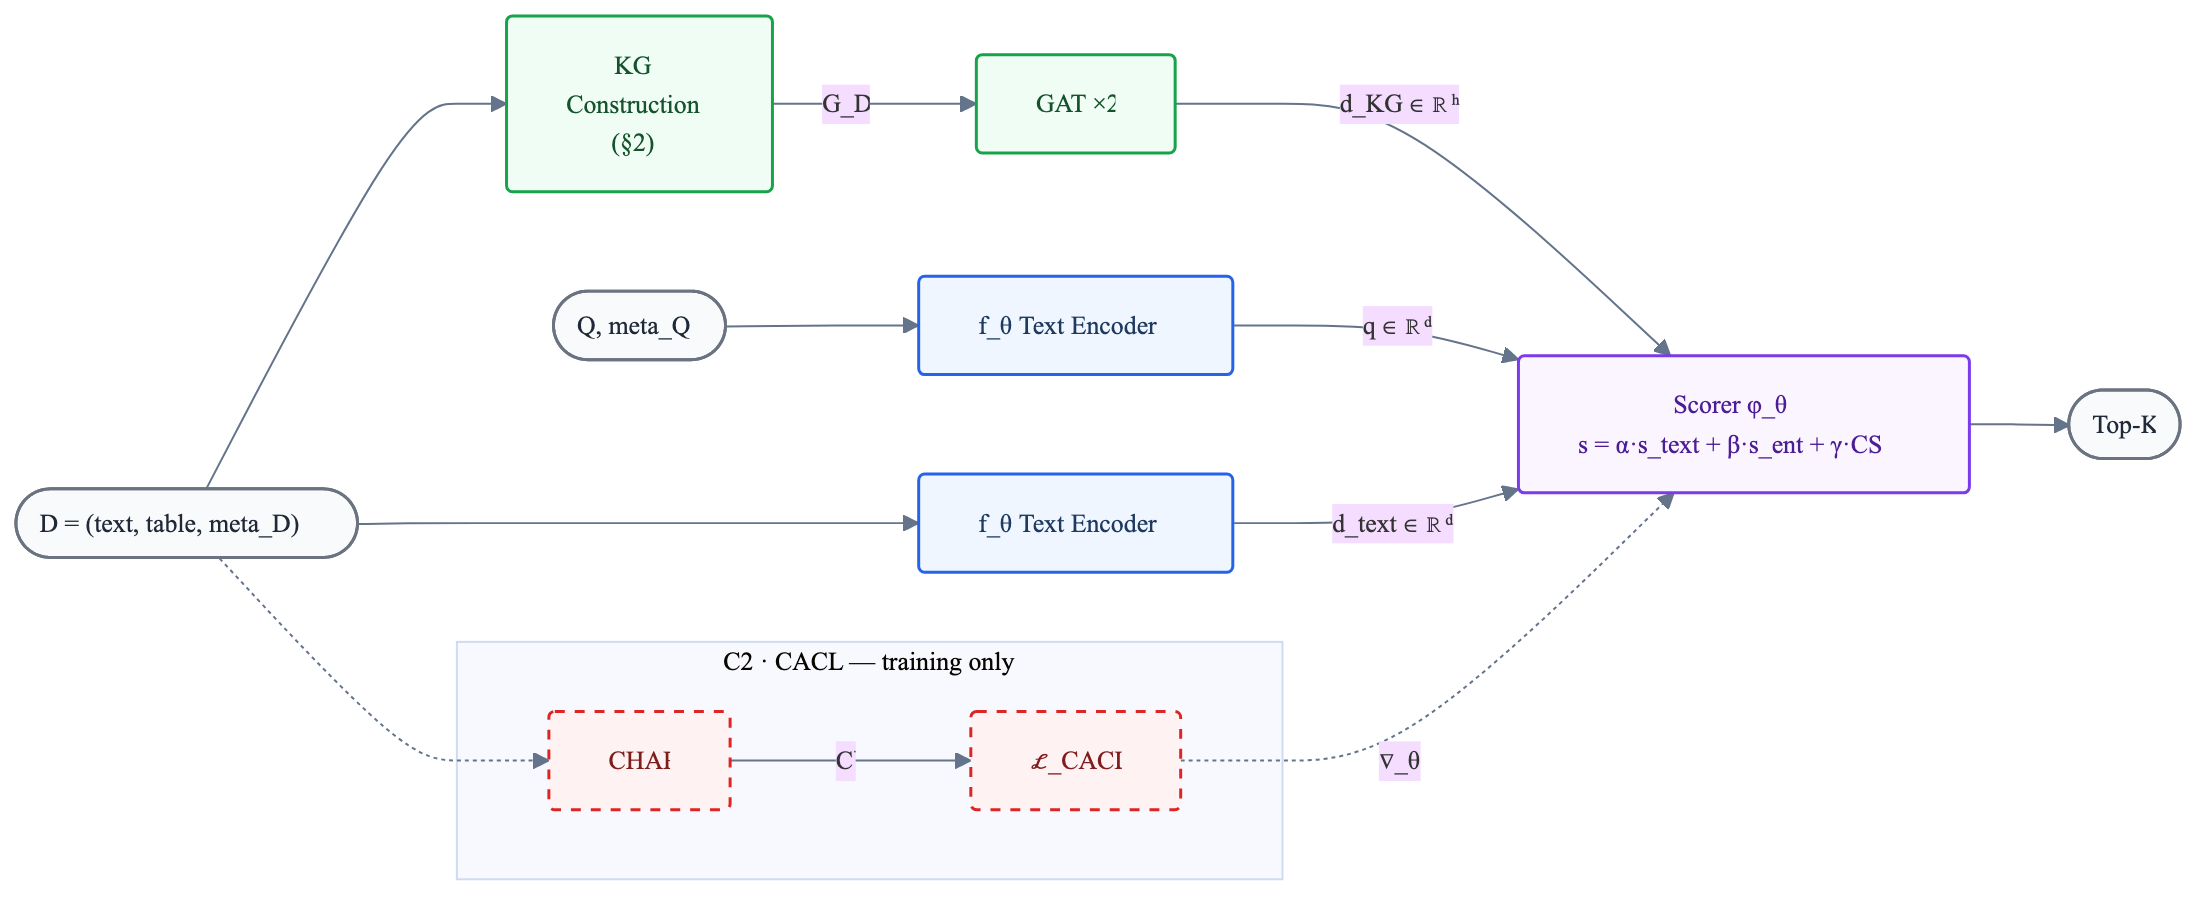
\includegraphics[width=\textwidth]{fig1_framework.png}
    \caption{GSR-CACL Framework. C1: Graph-Structured Retrieval (inference). C2: Constraint-Aware Contrastive Learning (training). Cả hai chia sẻ Joint Scorer $\phi_\theta$.}
    \label{fig:framework}
\end{figure}

\textbf{Contribution 1 --- GSR (Graph-Structured Retrieval) --- Inference.} Thay vì coi bảng tài chính như văn bản phẳng, GSR biểu diễn mỗi bảng dưới dạng đồ thị tri thức $G_D = (\mathcal{V}, \mathcal{E}, \omega)$ với các nút là ô số và các cạnh là ràng buộc kế toán. Hàm chấm điểm $\phi_\theta$ kết hợp ba tín hiệu: tương đồng văn bản, khớp thực thể, và mức tuân thủ ràng buộc:
\begin{equation}\label{eq:joint}
    s(Q, C) = \alpha \cdot s_{\text{text}}(Q, C) + \beta \cdot s_{\text{ent}}(Q, C) + \gamma \cdot \text{CS}(G_D)
\end{equation}

\textbf{Contribution 2 --- CACL (Constraint-Aware Contrastive Learning) --- Training.} CACL huấn luyện $\phi_\theta$ bằng cách tạo mẫu âm khó (hard negatives) qua kỹ thuật CHAP -- phá vỡ có chủ đích đúng một đẳng thức kế toán. Hàm mất mát kết hợp:
\begin{equation}\label{eq:cacl}
    \mathcal{L}_{\text{CACL}} = \mathcal{L}_{\text{triplet}} + \lambda \cdot \mathcal{L}_{\text{constraint}}
\end{equation}

\textbf{Mối quan hệ:} GSR cung cấp cấu trúc đồ thị để CACL học từ; CACL cung cấp tín hiệu huấn luyện chất lượng cao để GSR cải thiện khả năng nhận biết ràng buộc.

\subsection{Template-Based KG Construction}\label{sec:kg}

\begin{figure}[H]
    \centering
    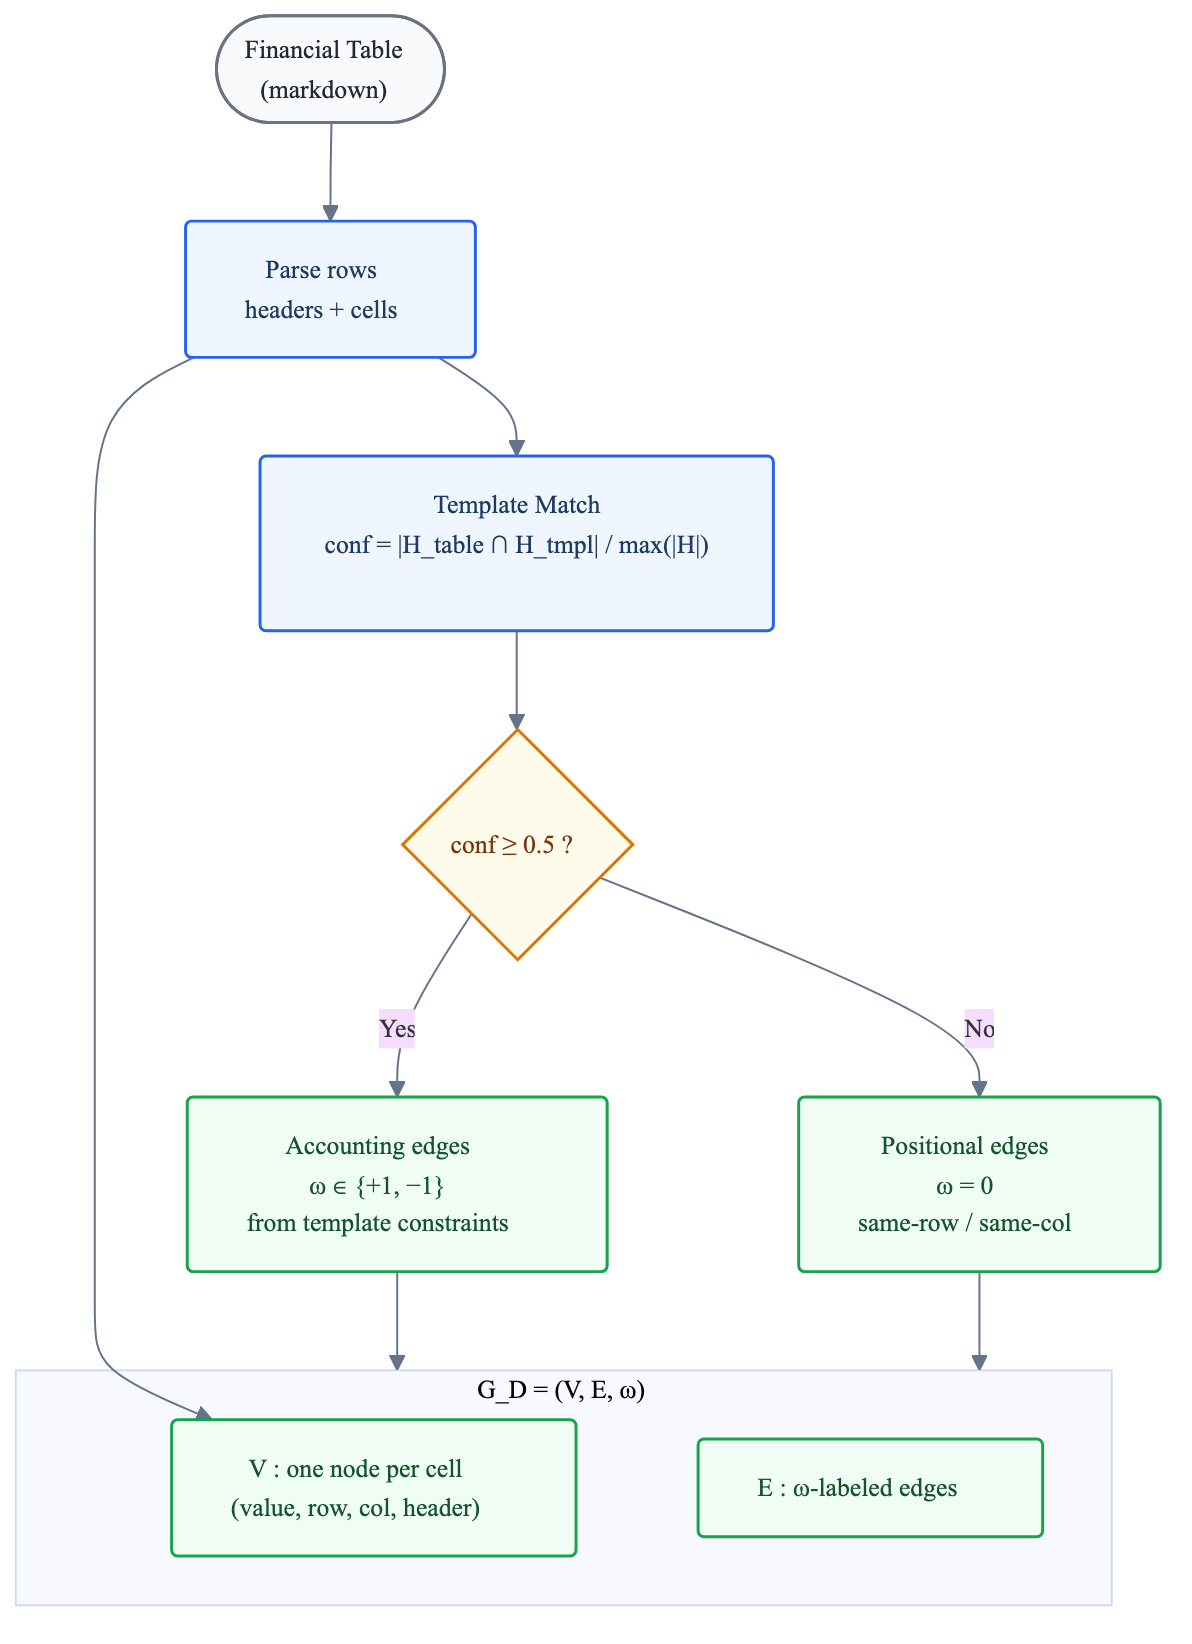
\includegraphics[width=0.7\textwidth]{fig2_kg_construction.png}
    \caption{Constraint KG Construction. Bảng tài chính được phân tích cú pháp, khớp với 15 template IFRS/GAAP, và chuyển đổi thành $G_D = (\mathcal{V}, \mathcal{E}, \omega)$.}
    \label{fig:kg}
\end{figure}

Mỗi bảng markdown $T$ được chuyển đổi thành đồ thị tri thức $G_D = (\mathcal{V}, \mathcal{E}, \omega)$ qua bốn bước:

\textbf{Bước 1 --- Parse.} Tách bảng thành tập header $\mathcal{H}$ và ma trận ô $\{c_{ij}\}$. Mỗi ô trở thành nút $v \in \mathcal{V}$ với thuộc tính $(\text{value}, \text{row}, \text{col}, \text{header})$.

\textbf{Bước 2 --- Template Matching.} So khớp $\mathcal{H}$ với thư viện $\mathcal{T}$ gồm 15 template IFRS/GAAP. Độ tin cậy:
\begin{equation}
    \text{conf}(\mathcal{H}, \tau) = \frac{|\{h \in \mathcal{H} \mid \text{normalize}(h) \in \mathcal{H}_\tau\}|}{\max(|\mathcal{H}|, |\mathcal{H}_\tau|)}, \quad \tau \in \mathcal{T}
\end{equation}

\begin{table}[H]
\centering\small
\begin{tabular}{ll}
\toprule
Template & Ràng buộc đại diện \\
\midrule
Income Statement & Revenue $-$ COGS $=$ Gross Profit; GP $-$ OpEx $=$ EBIT \\
Balance Sheet (Assets) & Current Assets $+$ Non-Current Assets $=$ Total Assets \\
Balance Sheet (L+E) & Total Liabilities $+$ Equity $=$ Total Assets \\
Cash Flow Statement & OCF $+$ ICF $+$ FCF $=$ Net Cash Flow \\
Revenue by Segment & $\sum_i$ Segment$_i$ $=$ Total Revenue \\
Quarterly Breakdown & Q1 $+$ Q2 $+$ Q3 $+$ Q4 $=$ Annual \\
\ldots{} (15 templates) & \ldots{} \\
\bottomrule
\end{tabular}
\end{table}

\textbf{Bước 3 --- Edge Construction.} Nếu $\text{conf} \geq \tau_{\min}$ (mặc định 0.5), tạo cạnh ràng buộc kế toán (accounting edges) với trọng số ngữ nghĩa:
\begin{equation}
    \omega_{uv} = \begin{cases} +1 & \text{nếu } v_u \text{ cộng vào } v_v \text{ (additive)} \\ -1 & \text{nếu } v_u \text{ trừ từ } v_v \text{ (subtractive)} \end{cases}
\end{equation}

\textbf{Bước 4 --- Fallback.} Nếu $\text{conf} < \tau_{\min}$, tạo cạnh vị trí (positional edges) $\omega = 0$ cho các ô cùng hàng/cùng cột.

\textbf{Coverage estimate:} $\sim$80--90\% bảng trong FinQA/ConvFinQA và $\sim$70\% trong TAT-DQA khớp ít nhất một template (sẽ được kiểm chứng trong \S6.5).

\subsection{Edge-Aware GAT Encoder}\label{sec:gat}

\begin{figure}[H]
    \centering
    \begin{subfigure}[b]{0.55\textwidth}
        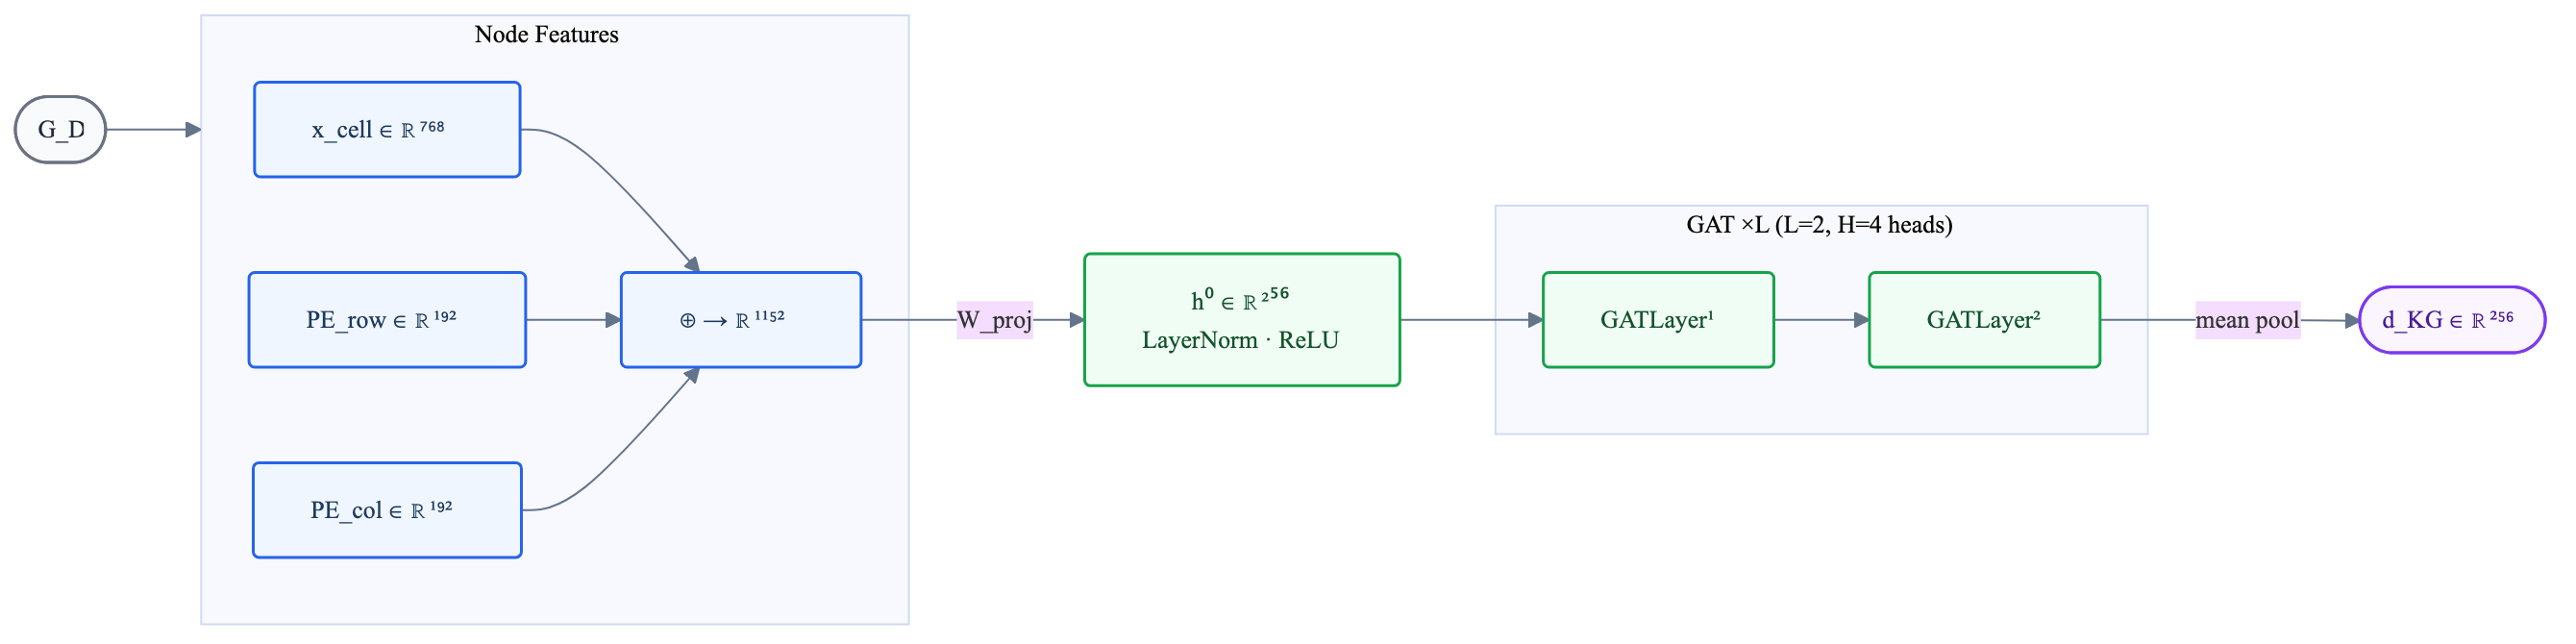
\includegraphics[width=\textwidth]{fig3_gat_encoder.png}
        \caption{GAT Encoder overview.}
    \end{subfigure}
    \hfill
    \begin{subfigure}[b]{0.42\textwidth}
        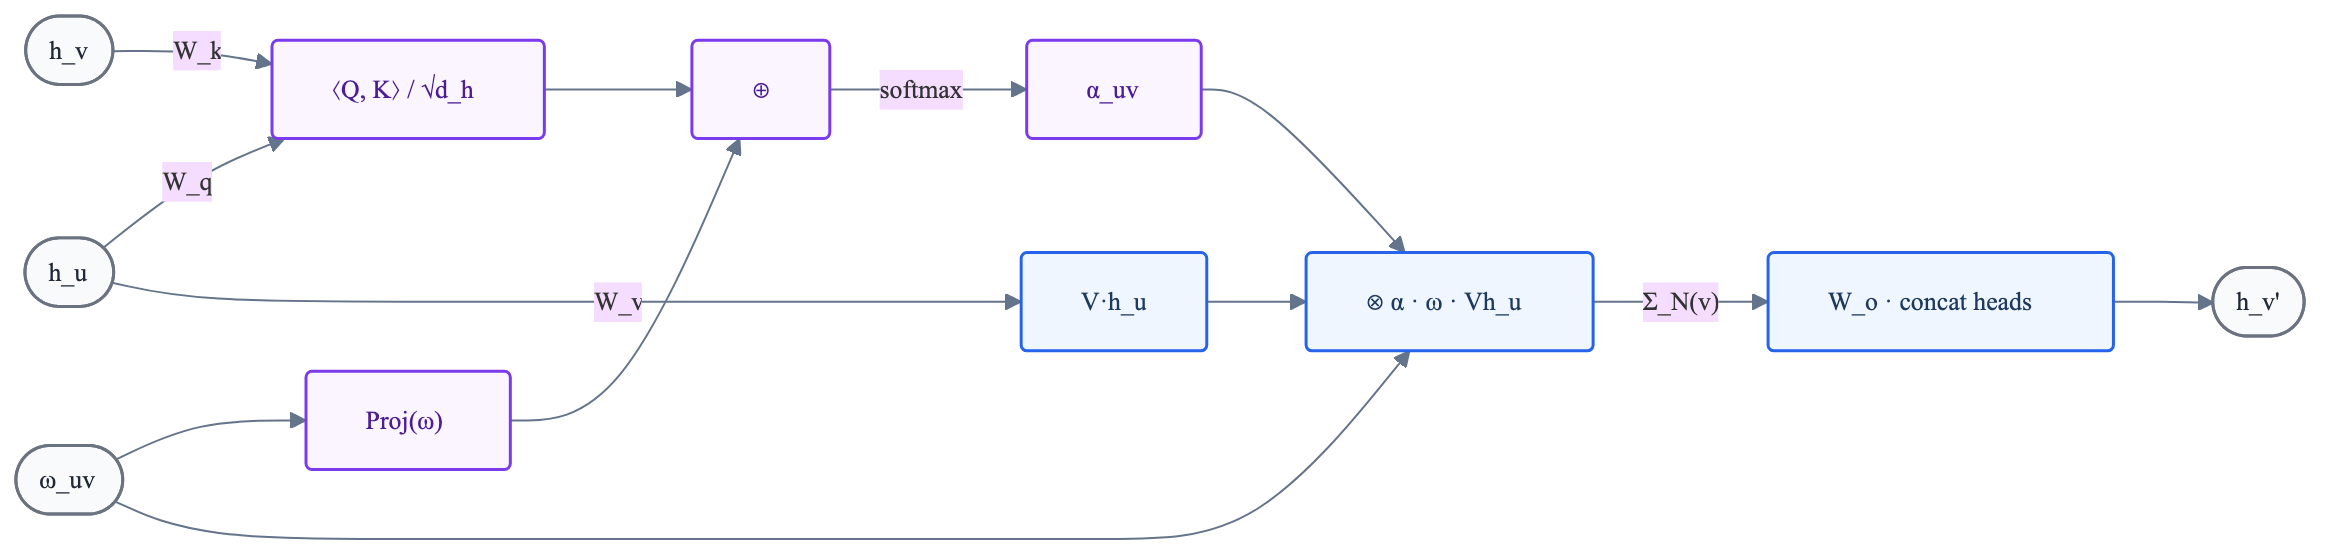
\includegraphics[width=\textwidth]{fig3b_edge_attention.png}
        \caption{Edge-aware attention detail.}
    \end{subfigure}
    \caption{GAT Encoder. (a)~Node features được chiếu qua $L{=}2$ edge-aware GAT layers, sau đó mean-pooled thành $\mathbf{d}_{\text{KG}}$. (b)~Mỗi attention head được bias bởi constraint weight $\omega$.}
    \label{fig:gat}
\end{figure}

\textbf{Node Feature Construction.} Mỗi nút $v$ tại vị trí $(r, c)$ được biểu diễn bằng phép nối:
\begin{equation}
    \mathbf{x}_v = f_\theta(\text{cell\_text}_v) \oplus \text{PE}_{\text{row}}(r) \oplus \text{PE}_{\text{col}}(c) \in \mathbb{R}^{d + 2p}
\end{equation}

trong đó $f_\theta$ là text encoder, $\text{PE}$ là mã hóa vị trí dạng sinusoidal với $p = d/4$. Phép chiếu đầu vào:
\begin{equation}
    \mathbf{h}_v^{(0)} = \text{ReLU}\big(\text{LayerNorm}(W_{\text{proj}}\, \mathbf{x}_v + b_{\text{proj}})\big) \in \mathbb{R}^{h_{\text{dim}}}
\end{equation}

\textbf{Edge-Aware Multi-Head Attention.} Tại mỗi layer $l$, mỗi head $k \in \{1,\ldots,H\}$ tính attention có thiên hướng theo trọng số ràng buộc $\omega$:
\begin{equation}
    e_{uv}^{(k)} = \frac{\langle W_q^{(k)} \mathbf{h}_u^{(l)},\; W_k^{(k)} \mathbf{h}_v^{(l)} \rangle}{\sqrt{d_k}} + \text{Proj}(\omega_{uv})
\end{equation}
\begin{equation}
    \alpha_{uv}^{(k)} = \frac{\exp(e_{uv}^{(k)})}{\sum_{w \in \mathcal{N}(v)} \exp(e_{wv}^{(k)})}
\end{equation}

\textbf{Message Passing \& Aggregation:}
\begin{equation}
    \mathbf{h}_v^{(l+1)} = W_o \bigg[\Big\|_{k=1}^{H} \sum_{u \in \mathcal{N}(v)} \alpha_{uv}^{(k)} \cdot \omega_{uv} \cdot W_v^{(k)} \mathbf{h}_u^{(l)} \bigg] + \mathbf{h}_v^{(l)}
\end{equation}

với residual connection. Kiến trúc: $L = 2$ layers, $H = 4$ heads, $h_{\text{dim}} = 256$.

\textbf{Graph-Level Representation.} Biểu diễn cấp tài liệu qua mean pooling:
\begin{equation}
    \mathbf{d}_{\text{KG}} = \frac{1}{|\mathcal{V}|} \sum_{v \in \mathcal{V}} \mathbf{h}_v^{(L)} \in \mathbb{R}^{h_{\text{dim}}}
\end{equation}

\subsection{Joint Scorer $\phi_\theta$}\label{sec:scorer}

\begin{figure}[H]
    \centering
    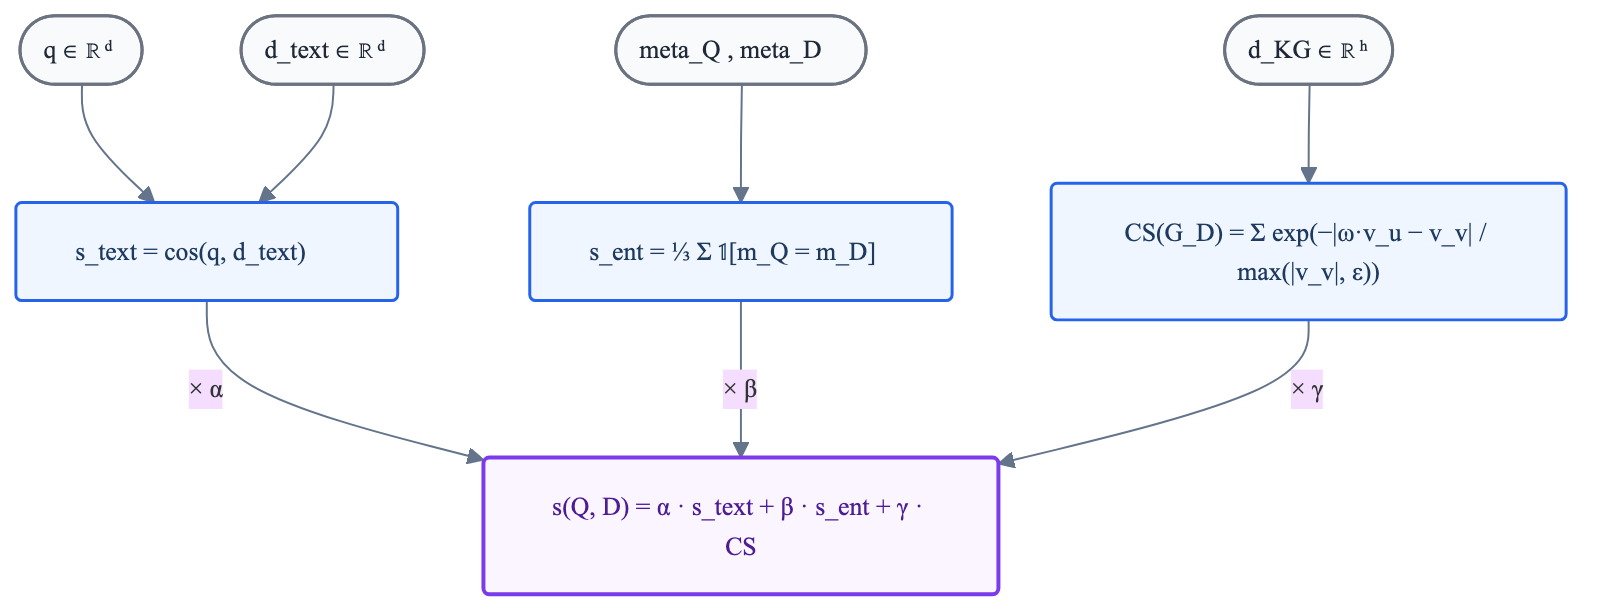
\includegraphics[width=0.6\textwidth]{fig4_joint_scorer.png}
    \caption{Joint Scorer. Ba tín hiệu bổ trợ --- văn bản, thực thể, cấu trúc --- được kết hợp qua trọng số dương học được $(\alpha, \beta, \gamma)$.}
    \label{fig:scorer}
\end{figure}

Hàm chấm điểm kết hợp ba tín hiệu bổ trợ (Eq.~\ref{eq:joint}), mỗi tín hiệu nắm bắt một khía cạnh khác nhau của sự liên quan:

\textbf{Text Similarity} --- Tương đồng ngữ nghĩa giữa câu hỏi và tài liệu:
\begin{equation}
    s_{\text{text}}(Q, C) = \cos(\mathbf{q}, \mathbf{d}_{\text{text}}) = \frac{\mathbf{q}^\top \mathbf{d}_{\text{text}}}{\|\mathbf{q}\| \cdot \|\mathbf{d}_{\text{text}}\|} \in [-1, 1]
\end{equation}

\textbf{Entity Score} --- Mức khớp siêu dữ liệu (công ty, năm, ngành):
\begin{equation}
    s_{\text{ent}}(Q, C) = \frac{1}{3} \sum_{k \in \{\text{co}, \text{yr}, \text{se}\}} \mathbb{1}[m_Q^k = m_C^k] \in [0, 1]
\end{equation}

\textbf{Constraint Score} --- Mức tuân thủ đẳng thức kế toán ($\varepsilon$-tolerance, differentiable):
\begin{equation}
    \text{CS}(G_D) = \frac{1}{|\mathcal{E}_c|} \sum_{(u,v,\omega) \in \mathcal{E}_c} \exp\!\left(-\frac{|\omega \cdot v_u - v_v|}{\max(|v_v|, \varepsilon)}\right) \in (0, 1]
\end{equation}

\textbf{Trọng số học được:} $\alpha = \text{softplus}(\log\hat{\alpha})$, $\beta = \text{softplus}(\log\hat{\beta})$, $\gamma = \text{softplus}(\log\hat{\gamma})$ --- luôn dương. Giá trị khởi tạo: $\alpha_0 = 0.5$, $\beta_0 = 0.3$, $\gamma_0 = 0.2$.

\subsection{CHAP: Constraint-Aware Hard Negative Generation}\label{sec:chap}

\begin{figure}[H]
    \centering
    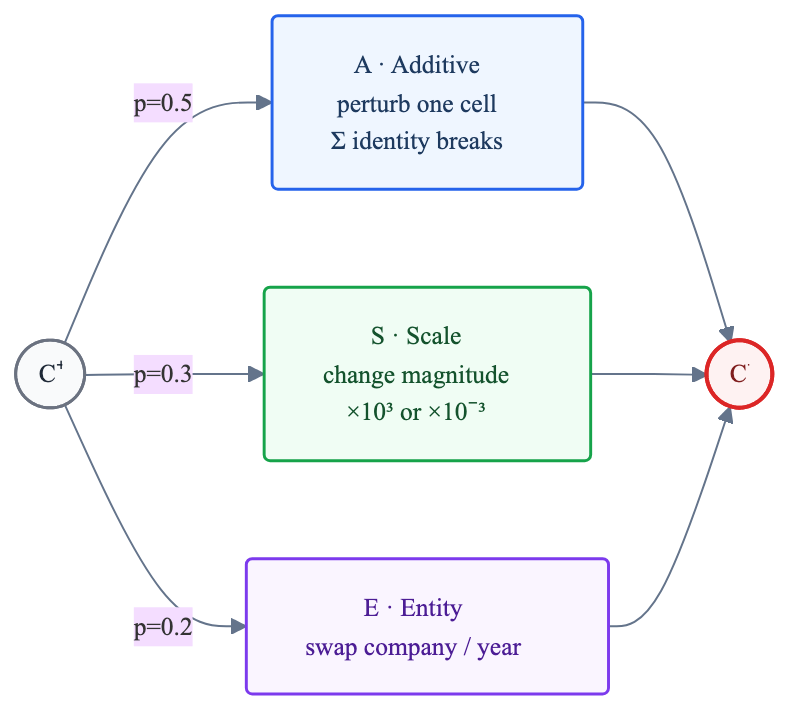
\includegraphics[width=0.7\textwidth]{fig5_chap.png}
    \caption{CHAP Negative Sampler. Ba kiểu nhiễu loạn, mỗi kiểu phá vỡ đúng một đẳng thức kế toán.}
    \label{fig:chap}
\end{figure}

Thay vì mẫu âm ngẫu nhiên (DPR~\cite{karpukhin2020dpr}) hoặc BM25 hard negatives, CHAP tạo mẫu âm $C^-$ từ tài liệu dương $C^+$ bằng cách phá vỡ có chủ đích \textbf{đúng một} đẳng thức kế toán. Ba kiểu nhiễu loạn:

\begin{table}[H]
\centering\small
\begin{tabular}{llll}
\toprule
Kiểu & Phép biến đổi & Ràng buộc bị vi phạm & Xác suất \\
\midrule
\textbf{A} (Additive) & Thay đổi 1 ô con, giữ nguyên ô tổng & $\sum_i v_{\text{child}_i} \neq v_{\text{parent}}$ & $p = 0.5$ \\
\textbf{S} (Scale) & Biến đổi bậc đại lượng ($\times 10^3$ hoặc $\times 10^{-3}$) & Tỷ lệ giữa các ô bị phá vỡ & $p = 0.3$ \\
\textbf{E} (Entity) & Hoán đổi company/year trong metadata & Sai khớp thực thể/thời gian & $p = 0.2$ \\
\bottomrule
\end{tabular}
\end{table}

\textbf{Tính chất Zero-Sum:} Mỗi $C^-$ chỉ khác $C^+$ đúng một thành phần $\Rightarrow$ mẫu âm có độ tương đồng bề mặt rất cao nhưng \textbf{chắc chắn} vi phạm ít nhất một ràng buộc. Điều này buộc mô hình phải học phân biệt dựa trên cấu trúc, không phải từ vựng.

\subsection{Training Objective: $\mathcal{L}_{\text{CACL}}$}\label{sec:loss}

\begin{figure}[H]
    \centering
    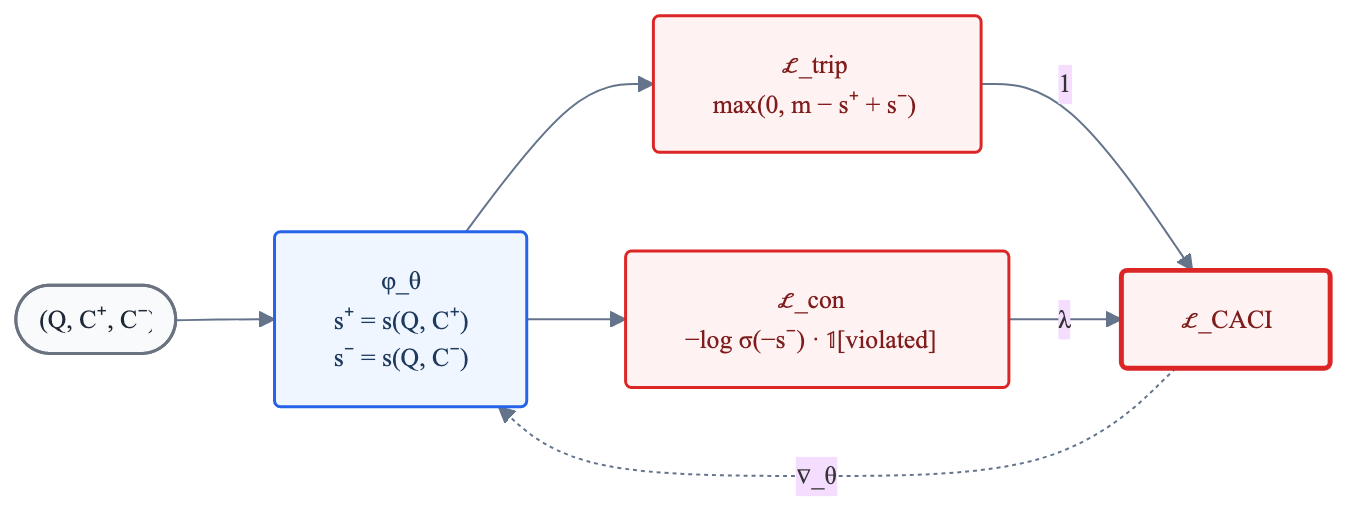
\includegraphics[width=0.7\textwidth]{fig6_cacl_loss.png}
    \caption{CACL Training Objective. Kết hợp margin-based triplet loss với constraint violation penalty.}
    \label{fig:loss}
\end{figure}

Hàm mất mát kết hợp hai thành phần (Eq.~\ref{eq:cacl}):

\textbf{Triplet Loss} --- Đẩy điểm tài liệu dương cao hơn tài liệu âm một khoảng margin $m$:
\begin{equation}
    \mathcal{L}_{\text{triplet}} = \frac{1}{N} \sum_{i=1}^{N} \max\!\big(0,\; m - s(Q_i, C_i^+) + s(Q_i, C_i^-)\big)
\end{equation}

\textbf{Constraint Violation Loss} --- Phạt nặng khi mô hình gán điểm cao cho tài liệu vi phạm ràng buộc:
\begin{equation}
    \mathcal{L}_{\text{constraint}} = -\frac{1}{N} \sum_{i=1}^{N} \mathbb{1}[\text{violated}(C_i^-, G_{C_i^-})] \cdot \log\sigma(-s(Q_i, C_i^-))
\end{equation}

\textbf{Trực giác:} $\mathcal{L}_{\text{triplet}}$ dạy mô hình phân biệt đúng/sai; $\mathcal{L}_{\text{constraint}}$ dạy mô hình \textit{tại sao} sai --- vì vi phạm ràng buộc kế toán. Siêu tham số $\lambda$ điều chỉnh cân bằng hai tín hiệu.

\subsection{Three-Stage Curriculum Training}\label{sec:curriculum}

\begin{figure}[H]
    \centering
    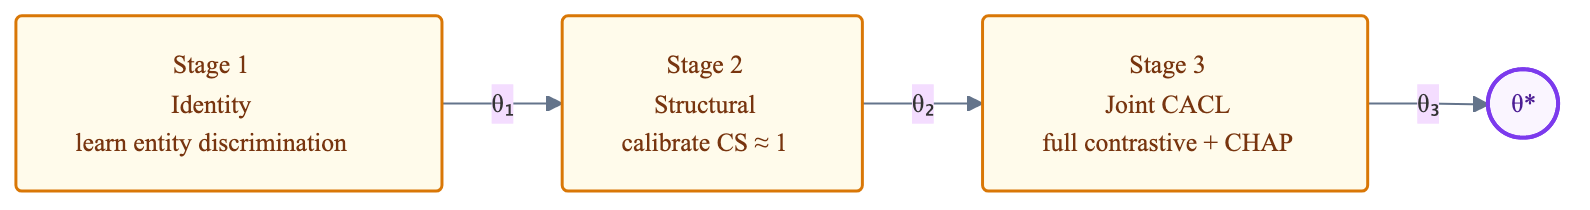
\includegraphics[width=0.7\textwidth]{fig7_curriculum.png}
    \caption{Three-Stage Curriculum. Trọng số được chuyển tuần tự $\theta_1 \to \theta_2 \to \theta_3 = \theta^*$.}
    \label{fig:curriculum}
\end{figure}

Huấn luyện theo chương trình (curriculum) ba giai đoạn, trọng số được chuyển tuần tự $\theta_1 \to \theta_2 \to \theta_3 = \theta^*$:

\begin{table}[H]
\centering\small
\begin{tabular}{llll}
\toprule
Giai đoạn & Module được huấn luyện & Mục tiêu & Loss \\
\midrule
\textbf{Stage 1: Identity} & $f_\theta$ + $\phi_\theta$ (text + entity) & Học phân biệt $(company, year)$ & $\mathcal{L}_{\text{triplet}}$ (chỉ $s_{\text{text}} + s_{\text{ent}}$) \\
\textbf{Stage 2: Structural} & $f_\theta$ + GAT + $\phi_\theta$ & Hiệu chuẩn $\text{CS} \approx 1$ cho tài liệu hợp lệ & $\mathcal{L}_{\text{triplet}}$ (full $s$) \\
\textbf{Stage 3: Joint CACL} & $f_\theta$ + GAT + $\phi_\theta$ + CHAP & Tối ưu toàn diện với mẫu âm khó & $\mathcal{L}_{\text{CACL}}$ (Eq.~\ref{eq:cacl}) \\
\bottomrule
\end{tabular}
\end{table}

Mỗi giai đoạn cung cấp khởi tạo tốt hơn cho giai đoạn tiếp theo, tránh collapse khi huấn luyện toàn bộ từ đầu.

%% ============================================================
%% 5. EXPERIMENTAL SETUP
%% ============================================================
\section{Experimental Setup}

\subsection{Datasets}

Chúng tôi đánh giá trên $\mathrm{T}^{2}$-RAGBench~\cite{strich2026t2ragbench} --- benchmark chuẩn cho truy xuất tài liệu tài chính hỗn hợp văn bản-bảng, bao gồm ba tập con:

\begin{table}[H]
\centering\small
\begin{tabular}{lrrrr}
\toprule
Subset & Documents & QA Pairs & Avg. Token/Doc & Domain \\
\midrule
FinQA~\cite{chen2021finqa} & 2,789 & 8,281 & 950.4 & S\&P 500 financial reports \\
ConvFinQA~\cite{chen2022convfinqa} & 1,806 & 3,458 & 890.9 & S\&P 500 (conversational) \\
TAT-DQA~\cite{zhu2022tatdqa} & 2,723 & 11,349 & 915.3 & Diverse financial reports \\
\midrule
\textbf{Tổng} & \textbf{7,318} & \textbf{23,088} & \textbf{924.2} & \\
\bottomrule
\end{tabular}
\caption{Thống kê $\mathrm{T}^{2}$-RAGBench. Mỗi mẫu là bộ ba $(Q, A, C)$ với câu hỏi context-independent đã được xác nhận bởi chuyên gia (91.3\% context-independent, Cohen's $\kappa = 0.87$). Câu hỏi yêu cầu truy xuất ngữ cảnh đúng trước khi thực hiện suy luận số học.}
\end{table}

\subsection{Baselines}

Các baselines được phân nhóm theo chiến lược truy xuất để tạo bối cảnh đối chiếu công bằng:

\textbf{Nhóm 1 --- Giới hạn trên/dưới (Bounds):}

\begin{table}[H]
\centering\small
\begin{tabular}{ll}
\toprule
Phương pháp & Mô tả \\
\midrule
Pretrained-Only & Không dùng retriever, LLM trả lời từ pre-training knowledge \\
Oracle Context & Ngữ cảnh đúng được cung cấp trực tiếp (giới hạn trên) \\
\bottomrule
\end{tabular}
\end{table}

\textbf{Nhóm 2 --- Basic RAG Methods:}

\begin{table}[H]
\centering\small
\begin{tabular}{ll}
\toprule
Phương pháp & Mô tả \\
\midrule
Base-RAG~\cite{karpukhin2020dpr} & Dense retrieval chuẩn (embed query $\to$ cosine similarity) \\
Hybrid BM25 & Kết hợp sparse (BM25) + dense retrieval --- \textbf{best reported} trên $\mathrm{T}^{2}$-RAGBench \\
Reranker & Cross-encoder reranking sau initial retrieval \\
\bottomrule
\end{tabular}
\end{table}

\textbf{Nhóm 3 --- Advanced RAG Methods:}

\begin{table}[H]
\centering\small
\begin{tabular}{ll}
\toprule
Phương pháp & Mô tả \\
\midrule
HyDE & Sinh câu trả lời giả $\to$ dùng làm query mới \\
Summarization & Tóm tắt ngữ cảnh trước khi retrieval \\
SumContext & Retrieval từ bản tóm tắt, nhưng trả về ngữ cảnh gốc đầy đủ \\
\bottomrule
\end{tabular}
\end{table}

\textbf{Nhóm 4 --- Table-Aware Methods (SOTA cho bảng):}

\begin{table}[H]
\centering\small
\begin{tabular}{ll}
\toprule
Phương pháp & Mô tả \\
\midrule
THoRR~\cite{thorr2024} & Two-stage retrieval dựa trên header concatenation \\
ConFIT~\cite{confit2025} & Semantic-Preserving Perturbation --- so sánh trực tiếp với CHAP \\
\bottomrule
\end{tabular}
\end{table}

\textbf{Nhóm 5 --- Our Methods:}

\begin{table}[H]
\centering\small
\begin{tabular}{ll}
\toprule
Phương pháp & Mô tả \\
\midrule
GSR & Graph-Structured Retrieval (Contribution 1) \\
GSR + CACL & Full system với CHAP training (Contribution 1 + 2) \\
HybridGSR & GSR + BM25 + Reciprocal Rank Fusion \\
\bottomrule
\end{tabular}
\end{table}

\subsection{Evaluation Metrics}

\begin{table}[H]
\centering\small
\begin{tabular}{lll}
\toprule
Metric & Ý nghĩa & Lý do lựa chọn \\
\midrule
\textbf{MRR@3} & Mean Reciprocal Rank tại $k{=}3$ & Metric chính của $\mathrm{T}^{2}$-RAGBench; đánh giá thứ hạng tài liệu đúng trong top-3 \\
\textbf{Recall@3} & Tỷ lệ câu hỏi có tài liệu đúng trong top-3 & Đánh giá coverage; giới hạn $k{=}3$ vì avg.\ doc length = 924 tokens \\
\textbf{NM (Number Match)} & Câu trả lời số đúng (tolerance $\varepsilon = 10^{-2}$, scale-invariant) & End-to-end metric: retrieval đúng $\to$ reasoning đúng \\
\textbf{Recall@1, Recall@5} & Supplementary recall tại $k{=}1$ và $k{=}5$ & Phân tích chi tiết chất lượng retrieval \\
\bottomrule
\end{tabular}
\caption{Chúng tôi tập trung vào \textbf{MRR@3 và R@3} cho retrieval evaluation (vì bài toán chính là retrieval), và báo cáo NM cho end-to-end reference.}
\end{table}

\subsection{Implementation Details}

\begin{table}[H]
\centering\small
\begin{tabular}{ll}
\toprule
Tham số & Giá trị \\
\midrule
Text encoder & BAAI/bge-large-en-v1.5 ($d = 1024$) \\
Fine-tuning strategy & LoRA ($r = 16$, $\alpha = 32$, target: $W_q, W_v$) \\
GAT layers / heads / hidden & $L = 2$ / $H = 4$ / $h_{\text{dim}} = 256$ \\
Positional encoding dim & $p = 192$ (sinusoidal) \\
Node feature input dim & $d + 2p = 1024 + 384 = 1408$ \\
Template library size & $|\mathcal{T}| = 15$ templates IFRS/GAAP \\
Template matching threshold & $\tau_{\min} = 0.5$ \\
Training stages (epochs) & Stage 1: 3 / Stage 2: 3 / Stage 3: 5 \\
Batch size & 8 (T4 GPU) hoặc 16 (A100) \\
Learning rate & $2 \times 10^{-5}$ (AdamW, cosine schedule) \\
Margin $m$ & 0.3 \\
Constraint weight $\lambda$ & 0.5 \\
CHAP ratios (A/S/E) & 0.5 / 0.3 / 0.2 \\
Optimizer & AdamW ($\beta_1 = 0.9$, $\beta_2 = 0.999$, weight decay $= 0.01$) \\
Hardware & NVIDIA T4 16GB (Kaggle) hoặc A100 40GB \\
\bottomrule
\end{tabular}
\end{table}

\textbf{Offline Pre-indexing:} KG construction và GAT encoding được thực hiện offline cho toàn bộ corpus. Tại inference, chỉ cần encode query và tra cứu.

\begin{table}[H]
\centering\small
\begin{tabular}{llr}
\toprule
Component & Complexity & Per-document avg. \\
\midrule
KG Construction & $O(|\mathcal{V}|)$ & $\sim$57 cells \\
GAT Encoding & $O(|\mathcal{V}| \cdot |\mathcal{E}|)$ & $|\mathcal{V}| \approx 57$, $|\mathcal{E}| \approx 10$ \\
Constraint Scoring & $O(|\mathcal{E}_c|)$ & $\sim$5--10 edges \\
CHAP Generation & $O(|\mathcal{V}|)$ & Pre-generated offline \\
\midrule
\textbf{Tổng inference overhead} & & $\sim$1.2--1.4$\times$ so với Base-RAG \\
\bottomrule
\end{tabular}
\end{table}

%% ============================================================
%% 6. EXPECTED RESULTS & ANALYSIS
%% ============================================================
\section{Expected Results \& Analysis}

\begin{tcolorbox}[colback=yellow!10!white, colframe=orange!80!black, title=Lưu ý]
Đây là proposal --- các bảng kết quả được thiết kế sẵn với baseline numbers từ $\mathrm{T}^{2}$-RAGBench~\cite{strich2026t2ragbench} (Table 3). Kết quả của phương pháp đề xuất (GSR, GSR+CACL, HybridGSR) sẽ được điền sau khi chạy thực nghiệm.
\end{tcolorbox}

\subsection{Main Results}

\textbf{Exp 1 --- So sánh toàn diện với baselines.} Bảng dưới đây báo cáo hiệu năng retrieval (MRR@3, R@3) và end-to-end (NM) trên ba tập con. Generator sử dụng Llama 3.3-70B.

\begin{table*}[h!]
\centering
\tiny\setlength{\tabcolsep}{4pt}
\begin{tabular}{ll|ccc|ccc|ccc|ccc}
\toprule
& \multirow{2}{*}{Phương pháp} & \multicolumn{3}{c|}{FinQA} & \multicolumn{3}{c|}{ConvFinQA} & \multicolumn{3}{c|}{TAT-DQA} & \multicolumn{3}{c}{W. Avg} \\
& & NM & MRR@3 & R@3 & NM & MRR@3 & R@3 & NM & MRR@3 & R@3 & NM & MRR@3 & R@3 \\
\midrule
\multicolumn{14}{l}{\textit{Giới hạn (Bounds)}} \\
& Pretrained-Only & 7.9 & --- & --- & 2.8 & --- & --- & 3.7 & --- & --- & 5.1 & --- & --- \\
& Oracle Context & 76.2 & 100 & 100 & 75.8 & 100 & 100 & 69.2 & 100 & 100 & 72.7 & 100 & 100 \\
\multicolumn{14}{l}{\textit{Basic RAG}} \\
& Base-RAG & 39.5 & 38.7 & 49.7 & 47.4 & 42.2 & 53.8 & 29.6 & 25.2 & 28.4 & 35.8 & 32.6 & 39.8 \\
& Hybrid BM25 & 41.7 & 40.0 & 53.0 & 50.3 & 43.5 & 57.2 & 37.4 & 29.2 & 44.4 & 40.9 & 35.2 & 49.4 \\
& Reranker & 32.4 & 29.0 & 36.2 & 37.3 & 32.3 & 40.5 & 27.0 & 22.8 & 28.4 & 30.5 & 26.4 & 33.0 \\
\multicolumn{14}{l}{\textit{Advanced RAG}} \\
& HyDE & 38.4 & 35.4 & 45.7 & 44.8 & 39.8 & 50.9 & 26.7 & 20.8 & 26.7 & 33.6 & 28.9 & 37.1 \\
& Summarization & 27.3 & 47.3 & 59.5 & 35.2 & 52.1 & 63.8 & 14.6 & 24.7 & 31.5 & 22.2 & 36.9 & 46.4 \\
& SumContext & 47.2 & 47.3 & 59.4 & 55.5 & 52.1 & 63.8 & 29.1 & 24.8 & 31.4 & 39.5 & 37.0 & 46.3 \\
\multicolumn{14}{l}{\textit{Table-Aware}} \\
& THoRR & --- & --- & --- & --- & --- & --- & --- & --- & --- & --- & --- & --- \\
& ConFIT & --- & --- & --- & --- & --- & --- & --- & --- & --- & --- & --- & --- \\
\multicolumn{14}{l}{\textit{Ours}} \\
& GSR & --- & --- & --- & --- & --- & --- & --- & --- & --- & --- & --- & --- \\
& GSR + CACL & --- & --- & --- & --- & --- & --- & --- & --- & --- & --- & --- & --- \\
& HybridGSR & --- & --- & --- & --- & --- & --- & --- & --- & --- & --- & --- & --- \\
\bottomrule
\end{tabular}
\caption{Kết quả retrieval chính. Baseline numbers từ $\mathrm{T}^{2}$-RAGBench (Llama~3.3-70B + E5-Large). Kết quả của chúng tôi (---) sẽ được điền sau khi chạy thực nghiệm. \textbf{Kỳ vọng:} GSR+CACL vượt Hybrid BM25 $\geq$5 điểm MRR@3 (W.~Avg), đặc biệt trên TAT-DQA nơi cấu trúc bảng phức tạp hơn. HybridGSR (kết hợp BM25 sparse signal) kỳ vọng đạt kết quả cao nhất.}
\label{tab:main}
\end{table*}

\textbf{Phân tích dự kiến:}
\begin{itemize}[leftmargin=*]
    \item \textit{Tại sao GSR vượt trội?} Nhờ Constraint Score phân biệt được tài liệu có cấu trúc toán học hợp lệ --- tín hiệu mà dense/sparse retriever bỏ qua.
    \item \textit{Tại sao TAT-DQA khó nhất?} Cấu trúc bảng đa dạng hơn, template coverage thấp hơn ($\sim$70\% vs $\sim$85\%).
    \item \textit{So sánh với SumContext:} SumContext đạt MRR@3 cao nhờ denoising, nhưng GSR+CACL kỳ vọng vượt nhờ tín hiệu cấu trúc mà summarization không bảo toàn.
\end{itemize}

\subsection{Ablation Study}

\textbf{Exp 2 --- Đóng góp của từng module.} Loại bỏ lần lượt từng thành phần đề xuất tại \S4 để đo mức sụt giảm hiệu năng, chứng minh không module nào bị ``thừa''.

\begin{table}[H]
\centering\small
\begin{tabular}{llccc}
\toprule
Variant & Thành phần bị loại & Kiểm chứng & MRR@3 (W.~Avg) & $\Delta$ MRR@3 \\
\midrule
GSR + CACL (full) & --- & --- & --- & --- \\
$-$ Constraint KG & Bỏ toàn bộ KG, chỉ dùng text + entity & H1 & --- & --- \\
$-$ Constraint Score & Giữ KG cho GAT nhưng bỏ $\gamma \cdot \text{CS}$ khỏi $\phi_\theta$ & H1 & --- & --- \\
$-$ GAT Encoder & Bỏ GAT, chỉ dùng text + entity + CS truyền thống & H2 & --- & --- \\
$-$ Entity Score & Bỏ $\beta \cdot s_{\text{ent}}$ khỏi $\phi_\theta$ & --- & --- & --- \\
$-$ CHAP $\to$ Random Neg. & Thay CHAP bằng random negatives & H3 & --- & --- \\
$-$ CHAP $\to$ BM25 Hard Neg. & Thay CHAP bằng BM25 hard negatives & H3 & --- & --- \\
$-$ $\mathcal{L}_{\text{constraint}}$ & Chỉ dùng $\mathcal{L}_{\text{triplet}}$ & --- & --- & --- \\
$-$ Curriculum (direct Stage 3) & Bỏ Stage 1 + 2, train trực tiếp Stage 3 & --- & --- & --- \\
\bottomrule
\end{tabular}
\caption{Ablation study design. \textbf{Kỳ vọng:} Mỗi dòng ablation đều cho thấy $\Delta$MRR@3 $< 0$, với: $-$ Constraint KG: sụt giảm lớn nhất $\Rightarrow$ chứng minh H1. $-$ CHAP $\to$ Random: sụt giảm đáng kể $\Rightarrow$ chứng minh H3. $-$ Curriculum: sụt giảm vừa phải $\Rightarrow$ curriculum giúp nhưng không critical.}
\label{tab:ablation}
\end{table}

\subsection{CHAP Negative Type Analysis}

\textbf{Exp 3 --- Đánh giá khả năng phân biệt trên từng loại mẫu âm.} Đo MRR@3 khi inference trên 3 loại negatives khác nhau:

\begin{table}[H]
\centering\small
\begin{tabular}{lcccc}
\toprule
Negative Source & Base-RAG & Hybrid BM25 & GSR & GSR+CACL \\
\midrule
Random negatives & --- & --- & --- & --- \\
BM25 hard negatives & --- & --- & --- & --- \\
CHAP negatives & --- & --- & --- & --- \\
\bottomrule
\end{tabular}
\caption{CHAP negative type analysis. \textbf{Kỳ vọng:} GSR+CACL đạt hiệu năng cao và đồng đều trên cả 3 loại $\Rightarrow$ mô hình đã học \textit{constraint semantics} thực sự, không chỉ overfit vào dạng negative cụ thể.}
\end{table}

\subsection{Cross-Domain Generalization}

\textbf{Exp 4 --- Đánh giá khả năng tổng quát hóa chéo.} Train trên FinQA + ConvFinQA (cùng nguồn FinTabNet), test trên TAT-DQA (nguồn khác, cấu trúc bảng đa dạng hơn).

\begin{table}[H]
\centering\small
\begin{tabular}{llccc}
\toprule
Train Set & Test Set & MRR@3 & R@3 & $\Delta$ vs.\ in-domain \\
\midrule
FinQA + ConvFinQA & TAT-DQA & --- & --- & --- \\
TAT-DQA & FinQA & --- & --- & --- \\
All (in-domain) & All (in-domain) & --- & --- & baseline \\
\bottomrule
\end{tabular}
\caption{Cross-domain generalization. \textbf{Kỳ vọng:} Nhờ template-based approach dựa trên chuẩn IFRS/GAAP, mô hình tổng quát hóa tốt giữa các nguồn dữ liệu tài chính --- template coverage là yếu tố quyết định.}
\end{table}

\subsection{Template Coverage Analysis}\label{sec:coverage}

\textbf{Exp 5 --- Kiểm chứng claim coverage.} Chạy template matching trên toàn bộ corpus để kiểm chứng ước lượng \S4.3.

\begin{table}[H]
\centering\small
\begin{tabular}{lcccc}
\toprule
Subset & Total Tables & Matched ($\geq \tau_{\min}$) & Coverage (\%) & Avg. Accounting Edges \\
\midrule
FinQA & --- & --- & --- & --- \\
ConvFinQA & --- & --- & --- & --- \\
TAT-DQA & --- & --- & --- & --- \\
\bottomrule
\end{tabular}
\caption{Template coverage analysis toàn corpus $\mathrm{T}^{2}$-RAGBench.}
\end{table}

\subsection{Error Analysis}

\textbf{Exp 6 --- Phân tích lỗi định tính.} Lấy mẫu ngẫu nhiên các trường hợp GSR + CACL truy xuất sai, phân loại theo nguyên nhân:

\begin{table}[H]
\centering\small
\begin{tabular}{llc}
\toprule
Loại lỗi & Mô tả & Tỷ lệ (\%) \\
\midrule
Template Miss & Bảng không khớp template nào $\to$ fallback positional & --- \\
Entity Confusion & Cùng công ty, khác năm (hoặc ngược lại) & --- \\
Numerical Ambiguity & Cùng con số xuất hiện ở nhiều ngữ cảnh & --- \\
Complex Table & Bảng lồng nhau / multi-level headers & --- \\
Text-Only Answer & Câu trả lời nằm trong narrative, không dùng bảng & --- \\
\bottomrule
\end{tabular}
\caption{Error taxonomy. \textbf{Mục tiêu:} Chỉ ra giới hạn cụ thể của phương pháp, gợi ý hướng cải tiến (mở rộng template library, multi-level table parsing).}
\end{table}

%% ============================================================
%% TÀI LIỆU THAM KHẢO
%% ============================================================
\begin{thebibliography}{13}

\bibitem{strich2026t2ragbench}
J.~Strich, E.~K.~Isgorur, M.~Trescher, C.~Biemann, and M.~Semmann.
\newblock $\mathrm{T}^2$-RAGBench: A Benchmark for Table-Text Retrieval in Financial Documents.
\newblock In \textit{Proc.\ EACL}, 2026.

\bibitem{helios2025}
HELIOS: Multi-hop QA over Financial Tables and Text.
\newblock In \textit{Proc.\ ACL}, 2025.

\bibitem{thyme2025}
THYME: Field-aware Hybrid Matching for Table Retrieval.
\newblock In \textit{Proc.\ EMNLP}, 2025.

\bibitem{thorr2024}
THoRR: Two-stage Table Retrieval with Header Concatenation, 2024.

\bibitem{confit2025}
ConFIT: Semantic-Preserving Perturbation for Hard Negative Mining, 2025.

\bibitem{karpukhin2020dpr}
V.~Karpukhin, B.~O\u{g}uz, S.~Min, P.~Lewis, L.~Wu, S.~Edunov, D.~Chen, and W.-t.~Yih.
\newblock Dense Passage Retrieval for Open-Domain Question Answering.
\newblock In \textit{Proc.\ EMNLP}, pp.\ 6769--6781, 2020.

\bibitem{halliday1994}
M.~A.~K.~Halliday.
\newblock \textit{An Introduction to Functional Grammar}.
\newblock Edward Arnold, 1994.

\bibitem{shannon1948}
C.~E.~Shannon.
\newblock A Mathematical Theory of Communication.
\newblock \textit{Bell System Technical Journal}, 27(3):379--423, 1948.

\bibitem{swales1990}
J.~M.~Swales.
\newblock \textit{Genre Analysis: English in Academic and Research Settings}.
\newblock Cambridge University Press, 1990.

\bibitem{cover2006}
T.~M.~Cover and J.~A.~Thomas.
\newblock \textit{Elements of Information Theory}.
\newblock Wiley, 2nd edition, 2006.

\bibitem{chen2021finqa}
Z.~Chen et al.
\newblock FinQA: A Dataset of Numerical Reasoning over Financial Data.
\newblock In \textit{Proc.\ EMNLP}, pp.\ 3697--3711, 2021.

\bibitem{chen2022convfinqa}
Z.~Chen et al.
\newblock ConvFinQA: Exploring the Chain of Numerical Reasoning in Conversational Finance Question Answering.
\newblock In \textit{Proc.\ EMNLP}, pp.\ 6279--6292, 2022.

\bibitem{zhu2022tatdqa}
F.~Zhu et al.
\newblock TAT-DQA: Question Answering over Financial Tables with Text and Tables.
\newblock In \textit{Proc.\ EMNLP}, 2022.

\end{thebibliography}

\end{document}
